\chapter{Advanced Encryption Standard (AES)}

\section{Caratteristiche}
Sviluppato dai due crittografi belgi Joan Daemen e Vincent Rijmen l'Advanced Encryption Standard (AES), conosciuto anche come Rijndael, di cui più propriamente è una specifica implementazione, è un algoritmo di cifratura a blocchi utilizzato come standard dal governo degli Stati Uniti d'America. 

\paragraph{}
Data la sua sicurezza e le sue specifiche pubbliche si presume che in un prossimo futuro venga utilizzato in tutto il mondo come è successo al suo predecessore, il Data Encryption Standard (DES) che ha perso poi efficacia per vulnerabilità intrinseche. AES è stato adottato dalla National Institute of Standards and Technology (NIST) e dalla US FIPS PUB nel novembre del 2001 dopo 5 anni di studi, standardizzazioni e selezione finale tra i vari algoritmi proposti.

\subsection{ La chiave di sessione}
AES  usa un \textbf{key schedule} per espandere una chiave primaria corta in un certo numero di chiavi di \textbf{ciclo} differenti. La lunghezza della chiave ricavata dipende dal livello di sicurezza con cui vogliamo criptare i dati.
\paragraph{}
Per il livello SECRET è sufficiente una chiave a 128 bit mentre per il livello Top secret si consigliano chiavi a 192 o 256 bit. Questo significa che per la prima volta il pubblico ha accesso ad una tecnologia crittografica che NSA ritiene adeguata per proteggere i documenti TOP SECRET. Si è discusso sulla necessità di utilizzare chiavi lunghe (192 o 256 bit) per i documenti TOP SECRET. Alcuni ritengono che questo indichi che l'NSA ha individuato un potenziale attacco che potrebbe forzare una chiave relativamente corta (128 bit), mentre la maggior parte degli esperti ritiene che le raccomandazioni della NSA siano basate principalmente sul volersi garantire un elevato margine di sicurezza per i prossimi decenni contro un potenziale attacco esaustivo.


\subsection{Lo stato}
A differenza di \textbf{Rijndael}, algoritmo da cui AES deriva e che utilizza blocchi multipli di 32 bit a partire da 128 fino ad arrivare a 256, AES utilizza matrici di 4x4 byte chiamate \textbf{stati}.
\paragraph{} Dati 16 bit di informazione \(b_0,b_1,...,b_15\), verranno disposti nella matrice come segue
\(
\begin{bmatrix}
b_0 & b_4 & b_8 & b_{12} \\
b_1 & b_5 & b_9 & b_{13} \\
b_2 & b_6 & b_{10} & b_{14} \\
b_3 & b_7 & b_{11} & b_{15}
\end{bmatrix}
\)

\section{Descrizione dell'algoritmo}
L'algoritmo sfrutta diverse funzioni che modificano i valori della matrice di stato mantenendone però la dimensione. 
\paragraph{}
L'AES effettua:
\begin{itemize}
\item 10 round per la chiave a 128 bit
\item 12 round per la chiave a 192 bit
\item 14 round per la chiave a 256 bit
\end{itemize}

Ogni round consiste in diversi step, ognuno dei quali contiene  a sua volta quattro diverse fasi, inclusa una che sfrutta la chiave di ciclo. Questo consente di passare da un testo in chiaro \textit{plaintext} a un testo cifrato \textit{ciphertest}.


\begin{enumerate}
\item \textbf{KeyExpansions} La chiave di cifratura viene espansa dal key schedule per generare una chiave più grande contenente tutte le chiavi di ciclo.
\item \textbf{Round iniziale}
\begin{enumerate}
\item \textit{AddRoundKey} Ogni byte dello stato viene combinato con il byte corrispondente della chiave di ciclo tramite uno XOR
\end{enumerate}
\item \textbf{Rounds}
\begin{enumerate}
\item \textit{SubBytes} Ogni byte viene sostituito con un altro secondo delle tabelle.
\item \textit{ShiftRows} Una trasposizione dove le ultime tre righe dello stato sono shiftate a sinistra un certo numero di volte.
\item \textit{MixColumns} Opera sulle colonne combinandone i byte.
\item \textit{AddRoundKey}
\end{enumerate}
\item \textbf{Round Finale (senza MixColumns)}
\begin{enumerate}
\item \textit{SubBytes}
\item \textit{ShiftRows}
\item \textit{AddRoundKey}
\end{enumerate}
\end{enumerate}




\subsection{AddRoundKey}
Nella fase AddRoundKey, la chiave di sessione viene combinata con lo stato. Per ogni round viene derivata una sottochiave dalla chiave originaria usando il key schedule; ogni sottochiave è della stessa dimensione dello stato. La sottochiave è aggiunta allo stato combinando ogni byte di questo con il corrispondente byte della chiave con uno \textbf{XOR}. 

\begin{figure}[H]
\centering
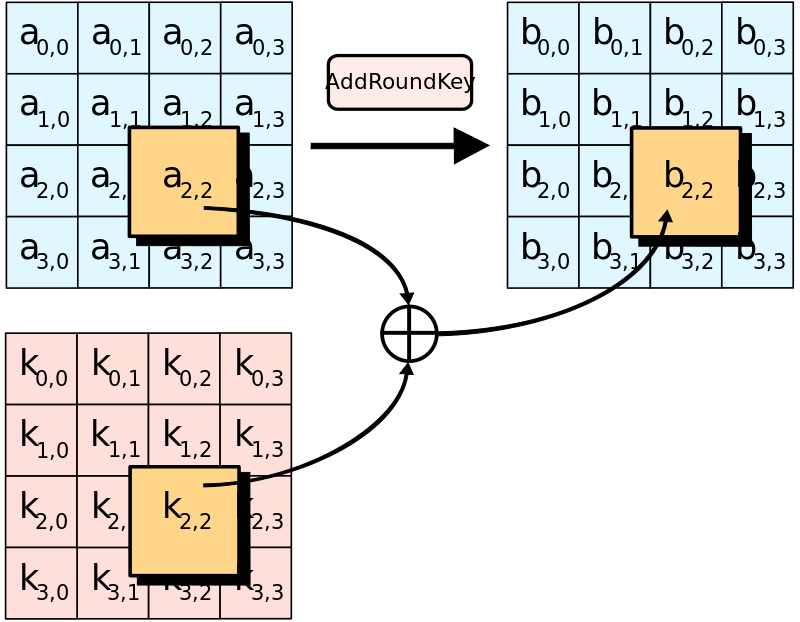
\includegraphics[scale=0.3]{img/addroundkey}
\caption{Nel passaggio AddRoundKeys ogni byte della matrice viene combinato con la sua sottochiave tramite un'operazione di XOR.}
\end{figure}

\subsection{SubBytes}
In SubBytes ogni byte \(a_{i,j}\) della matrice di stato è sostituito con il corrispondente byte di una matrice chiamata  \textbf{S-box}.
\begin{center}
\(b_{i,j} = S(a_{i,j})\)
\end{center}

Questa operazione garantisce la non-linearità della cifratura. 
La S-box utilizzata è derivata da una funzione inversa nel campo finito GF(\(2^8\)), conosciuta per avere delle ottime proprietà di non linearità. Per evitare un potenziale attacco basato sulle proprietà algebriche la S-box è costruita combinando la funzione inversa con una trasformazione affine invertibile. La S-box è stata scelta con cura per non possedere né punti fissi né punti fissi opposti.

\begin{figure}[H]
\centering
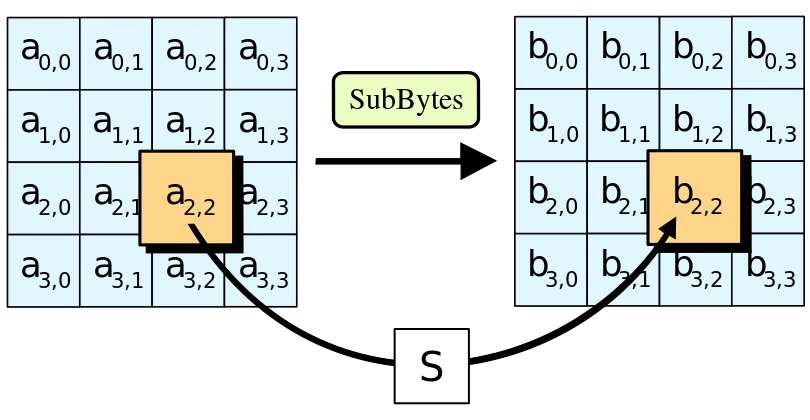
\includegraphics[scale=0.3]{img/subBytes}
\caption{Nel passaggio SubBytes, ogni byte della matrice è sostituito con i dati contenuti nella trasformazione S; \(b_{ij} = S(a_{ij})\).}
\end{figure}

\subsection{ShiftRows}
ShiftRows opera sulle righe dello stato shiftando ciclicamente i byte di ogni riga di un certo offset dipendente dal numero di riga lasciando la prima riga invariata.
Ogni byte della seconda riga è ciclicamente spostato a sinistra di una posizione. Similmente i byte della terza riga sono shiftati ciclicamente a sinistra di due posizioni e quelli della quarta di tre. 

In questo modo l'ultima colonna dei dati in ingresso andrà a formare la diagonale della matrice in uscita. (Rijndael utilizza un disegno leggermente diverso per via delle matrici di lunghezza non fissa.)


\begin{figure}[H]
\centering
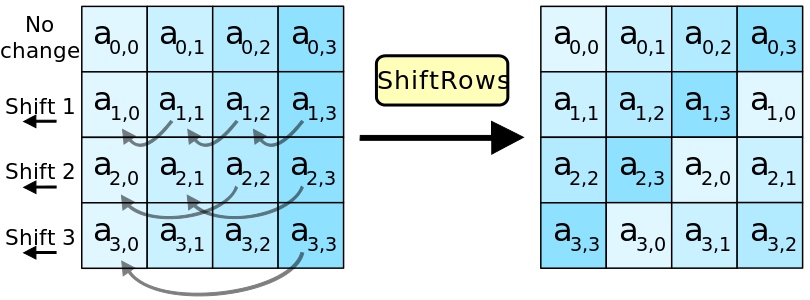
\includegraphics[scale=0.3]{img/shiftRows}
\caption{Nel passaggio ShiftRows, i byte di ogni riga vengono spostati verso sinistra dell'ordine della riga. Vedi figura per i singoli spostamenti.}
\end{figure}

\subsection{MixColumns}
Il passaggio MixColumns prende i quattro byte di ogni colonna e li combina utilizzando una trasformazione lineare invertibile. Utilizzati in congiunzione, ShiftRows e MixColumns provvedono a far rispettare il criterio di confusione e diffusione nell'algoritmo (teoria di Shannon). Ogni colonna è trattata come un polinomio in \(GF(2^8)\) e viene moltiplicata modulo \(x^4+1\) per un polinomio fisso \(c(x)=3x^3+x^2+x+2\).

\begin{figure}[H]
\centering
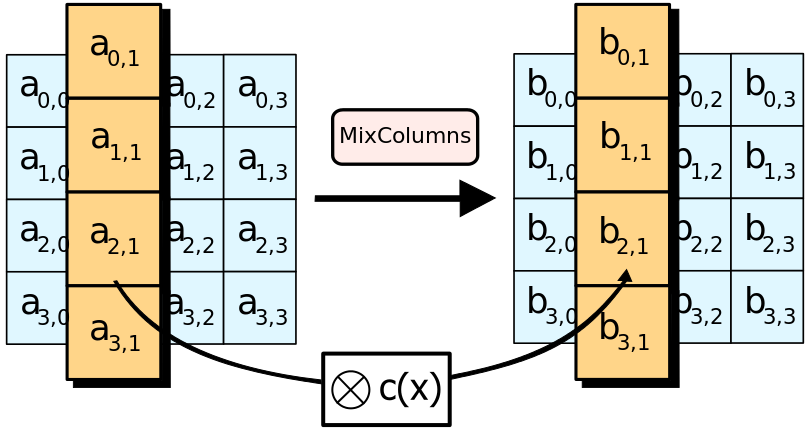
\includegraphics[scale=0.3]{img/mixColumns}
\caption{Nel passaggio MixColumns ogni colonna di byte viene moltiplicata per un polinomio fisso \(c(x)\).}
\end{figure}
